\subsection{Přeložení a sestavení programu}
Postup pro přeložení a sestavení je na všech platformách stejný. Je nutné mít nainstalovaný překladač \verb|gcc| a nástroj \verb|make| a mít zprovozněné jejich ekvivalentní příkazy v konzoli. Samotný překlad a sestavení provedeme v příkazovém řádku v kořenové složce programu příkazem \verb|make|. Po úspěšném sestavení se ve stejném adresáři vytvoří spustitelný binární soubor \verb|calc.exe|.

\begin{figure}[ht]
    \centering
    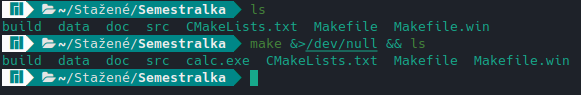
\includegraphics[width=0.8\textwidth]{sestaveni.png}
    \caption{Ukázka překladu a sestavení programu}\label{fig:sestaveni}
\end{figure}

\subsection{Spuštění a ovládání programu}
Program spouštíme, podle zadání, dvěma způsoby. 

Příkazem \verb|calc.exe| program otevřeme v interaktivním režimu (viz obr.~\ref{fig:ukazka_interaktivni}) pro postupné zadávání příkazů nebo infixových výrazů z příkazové řádky. Zadáním nepodporovaného příkazu nebo výrazu se špatnou syntaxí vypíše program odpovídající chybovou hlášku a čeká na nový příkaz. Příkazem \verb|quit| program ukončíme.

Příkazem \verb|calc.exe [<vstupni-soubor>]| program načte vstupní soubor, každý řádek v něm zpracuje jako zadaný výraz, řádek vypíše jako bychom ho zadali v interaktivním režímu a následně vypíše výsledek zpracování (viz obr.~\ref{fig:ukazka_soubor}). Po zpracování všech řádků v souboru se program ukončí s návratovou hodnotou \verb|EXIT_SUCCESS|. Pokud zadaný soubor neexistuje vypíše chybovou hlášku a skončí s návratovou hodnotou \verb|EXIT_FAILURE|. 
\newpage
\begin{figure}[ht]
    \centering
    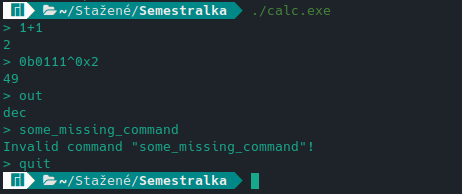
\includegraphics[width=0.8\textwidth]{ukazka_interaktivni.png}
    \caption{Ukázka interaktivního režimu}\label{fig:ukazka_interaktivni}
\end{figure}
\begin{figure}[ht]
    \centering
    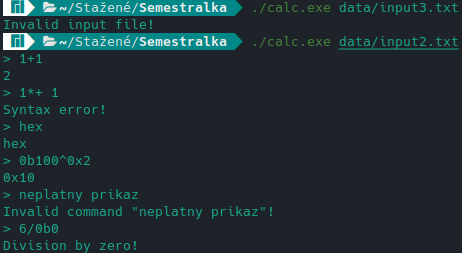
\includegraphics[width=0.8\textwidth]{ukazka_soubor.png}
    \caption{Ukázka načtení a zpracování souboru}\label{fig:ukazka_soubor}
\end{figure}